%%%%%%%%%%%%%%%%%%%%%%%%%%%%%%%%%%%%%%%%%%%%%%%%%%%%%%%%%%%%%%%%%%%%%%%%%%%%%%%%
%2345678901234567890123456789012345678901234567890123456789012345678901234567890
%        1         2         3         4         5         6         7         8

\documentclass[letterpaper, 10 pt, conference]{ieeeconf}  % Comment this line out
                                                          % if you need a4paper
%\documentclass[a4paper, 10pt, conference]{ieeeconf}      % Use this line for a4
                                                          % paper

\IEEEoverridecommandlockouts                              % This command is only
                                                          % needed if you want to
                                                          % use the \thanks command
\overrideIEEEmargins
% See the \addtolength command later in the file to balance the column lengths
% on the last page of the document



% The following packages can be found on http:\\www.ctan.org
%\usepackage{graphics} % for pdf, bitmapped graphics files
%\usepackage{epsfig} % for postscript graphics files
%\usepackage{mathptmx} % assumes new font selection scheme installed
%\usepackage{times} % assumes new font selection scheme installed
\usepackage{caption}
\usepackage{subfig}
\usepackage{amsmath} % assumes amsmath package installed
\usepackage{bm}
\usepackage{amssymb}  % assumes amsmath package installed
\usepackage{boldline}
\usepackage{array,multirow}
\usepackage{hyperref}
\usepackage{color}
\usepackage{graphicx}
\graphicspath{ {images/} }
\definecolor{light-gray}{gray}{0.95}
\newcommand{\code}[1]{\colorbox{light-gray}{\texttt{#1}}}
\DeclareMathOperator*{\argmax}{arg\,max}
\DeclareMathOperator*{\maxU}{max}
\usepackage{makecell}
\usepackage{bbm}
\usepackage[table,xcdraw]{xcolor}
\usepackage[flushleft]{threeparttable}
\usepackage[utf8]{inputenc}
\usepackage{xfrac}
\usepackage{capt-of}
\usepackage{algorithm}
\usepackage[noend]{algpseudocode}


\title{
Executive Summary \\
\large Track 3: A Reproducibility Study Concerning \emph{On the Convergence Of Adam and Beyond} \\
by Sashank, Kale, Kumar; 2018.
}

\author{ 
	\parbox{2 in}{\centering Tamir Bennatan
         {\tt\small tamir.bennatan@mail.mcgill.ca\\}
         {\tt\small 260614526}}
         \hspace*{ 0.3 in}
         \parbox{2 in}{\centering L\'ea Collin
         {\tt\small lea.collin@mail.mcgill.ca\\}
         {\tt\small 260618407}}
         \hspace*{0.3 in}
         \parbox{2 in}{\centering Emmanuel Ng Cheng Hin
         {\tt\small emmanuel.ngchenghin@mail.mcgill.ca\\}
         {\tt\small 260615964}}
}



\begin{document}



\maketitle
\thispagestyle{empty}
\pagestyle{empty}

%%%%%%%%%%%%%%%%%%%%%%%%%%%%%%%%%%%%%%%%%%%%%%%%%%%%%%%%%%%%%%%%%%%%%%%%%%%%%%%%

\section{Overview}

In this study, we seek to assess the reproducibility of the results reported in the paper \emph{On the Convergence of Adam and Beyond} (Sashank, Kale \& Kumar; 2018). The authors of this paper discuss issues with a popular variant of stochastic gradient descent called \emph{Adam}, and propose an improved algorithm, \emph{AMSGrad}. In this paper, we recreate four experiments described by the authors - one using a synthetic dataset, and three using the MNIST and CIFAR-10 datasets. We report results that are less conclusive than those reported by the authors, and discuss details that were omitted from the original paper that hinder reproducibility of the authors' results.

\section{Methodology}

In our experiments, we aimed to be faithful to the experimental setups the authors describe. Although the authors do not include all the details regarding their experiments, we emulated every design choice the authors reported. We implemented all our classifiers using \texttt{keras} - which has implementations of the Adam and AMSGrad optimizers - and ran our grid searches using the \code{GridSearchCV} object and \code{KerasClassifier} wrapper from \texttt{sklearn}.

\section{Key Findings}

A brief overview of our results compared to the results of the paper can be seen in Figure 1. Overall, we observe similar trends in convergence behaviour between Adam and AMSGrad in all four experiment as the authors did. 

One thing to note is that the training and test losses in the paper and in our results do not appear to be on the same scale. Though our overall trends in difference in performance between ADAM and AMSGrad match those reported by the authors, we discuss the discrepancy and implications in the discussion. 

\section{Discussion}

Although the authors take care to justify their claims with theory, there are several issues with their methodology and presentation of results, making it difficult to recreate their experiments exactly. 

To start, the authors do not specify for how many epochs they trained each of the described classifiers. Although the results they provide [Figure 1] show the number of \emph{iterations} they trained for, it is difficult to decipher what these iterations actually represent. To circumvent this ambiguity, we determined a number of training epochs for each model that allowed the model to converge, while remaining within a reasonable time frame. 

As touched upon in the key findings, our training and test losses were not on the same scale as those of the authors'. This is due to the fact that the authors do not report which loss they use for their models. The natural choice in a multi-class classification setting is categorical cross entropy. After running our experiments using categorical cross entropy, however, we noticed that the scale of our models' losses did not match those reported by the authors. As an alternative, we tried using binary cross entropy. With this loss, we were able to get much closer to the scale achieved by the authors (with minor discrepancies). Though this prevented us from being able to reproduce the results of the authors exactly, we still observed the same relative magnitude of loss between Adam and AMSGrad. 

Furthermore, the authors do not report their fully tuned hyperparameters for each model. The authors mention that they tune the learning rate $\alpha$ using a grid search, yet they do not specify a range or which learning rate they ultimately used. This forced us to experiment with large parameter spaces when we recreated their grid searches. As training deep networks such as CifarNet is computationally intensive, exhaustive searches are costly. Thus, omitting the final hyperparameters introduces computational barriers to reproducing the authors' results. The grid search for CifarNet took about 28 hours to complete. This time could have been greatly reduced if the authors had given us the exact values of the best hyperparameters they found, or at least  a range for the $\alpha$ values they looked through. 

Finally, the authors present their results by displaying the loss trajectories during a single training run for each of the experiments described. As we found by training each model several times, there is variability between different training runs and in some, the difference in performance between Adam and AMSGrad was negligible. The only experiment in which we found that AMSGrad indubitably performs better than Adam is the synthetic experiment. This is unsurprising as the experiment was designed specifically for Adam to fail. Because the authors do not go into detail about how often these 'perfect' situations for Adam to fail arise in reality and there was usually little difference in performance between Adam and AMSGrad in the non-synthetic experiments, it difficult to determine from this paper how much AMSGrad is truly necessary. 


\begin{figure*}
  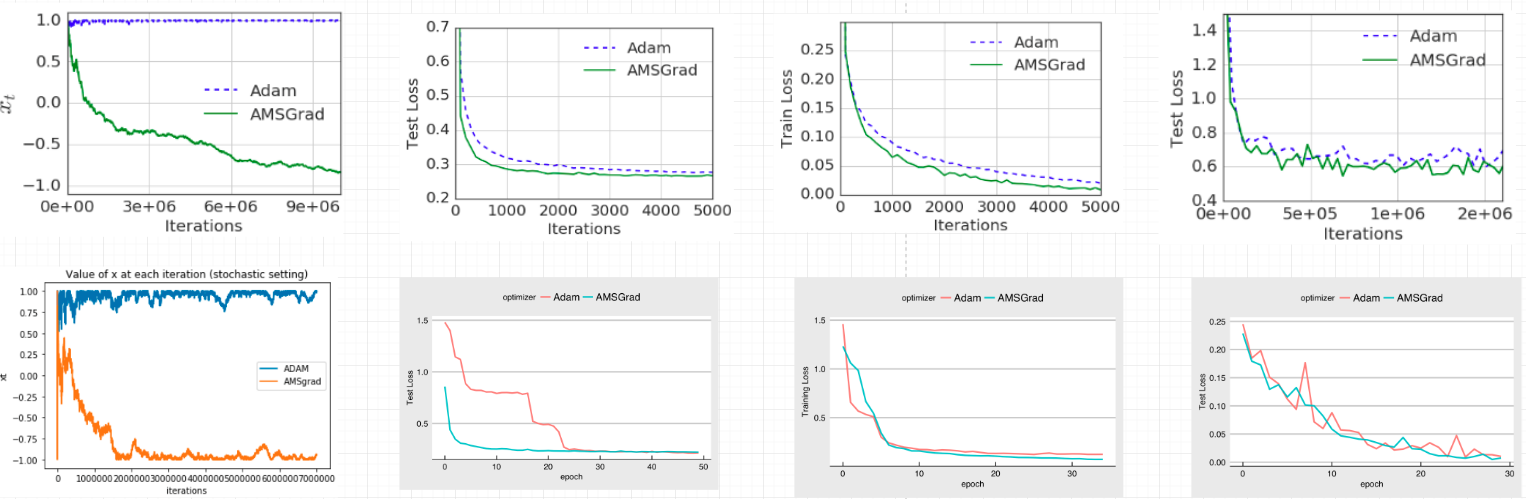
\includegraphics[width=1\linewidth]{ExecutiveSummaryResults.png}
  \label{fig:test2}
\caption[]{Top: The results from the original paper; (from left to right) location of $x_{t}$ in the stochastic synthetic experiments with respect to iterations, test loss of Adam and AMSGrad on logistic regression, training loss of Adam and AMSGrad with respect to iterations in 1-hidden layer feedforward neural network on MNIST, test loss of Adam and AMSGrad with respect to iterations for CifarNet \\
Bottom: Our results after attempting to reproduce; in the same order as top row}
\end{figure*}

For the full report on this paper, go to: \href{https://github.com/tamirbennatan/Adam-Convergence/blob/master/Report/FinalReport.pdf}{Final Report}
 
\addtolength{\textheight}{-12cm}   % This command serves to balance the column lengths
                                  % on the last page of the document manually. It shortens
                                  % the textheight of the last page by a suitable amount.
                                  % This command does not take effect until the next page
                                  % so it should come on the page before the last. Make
                                  % sure that you do not shorten the textheight too much.

%%%%%%%%%%%%%%%%%%%%%%%%%%%%%%%%%%%%%%%%%%%%%%%%%%%%%%%%%%%%%%%%%%%%%%%%%%%%%%%%

\end{document}

